\documentclass[MS]{inithesis}
%\documentclass[economy,twoside,bind]{inithesis}
% Use the second for a single-spaced copy suitable for duplex printing
% and binding.

% Other useful options (there are more options documented in Chapter 2):
%  * draft -- don't actually include images, print a black bar on overful
%             hboxes
%  * MS    -- Format for a Master's Thesis.  No UMI abstract page, some 
%             textual changes to title page.  


% Useful packages for thesis writing:
\usepackage{amsmath, amssymb, amsfonts, amsthm}
\usepackage{graphicx}
%\usepackage{natbib}
\usepackage{color}
\usepackage{bm}
%\usepackage{subfigure}
\usepackage{graphicx}
\usepackage{mathabx}
\usepackage{multirow}
\usepackage{setspace}
\usepackage{pdfpages}
\usepackage{tocloft}
\addtolength\cftfignumwidth{2.7em}%
\addtolength\cfttabnumwidth{2.7em}%
%\renewcommand{\cftpartnumwidth}{4em}
%\renewcommand{\cftchapaftersnumb}{\hspace{0em}}
%\renewcommand{\cftsecnumwidth}{1.5em}
%\renewcommand{\cftsecaftersnumb}{\hspace{0em}}
%\renewcommand{\cftsubsubsecindent}{8em}
%\renewcommand{\cftsubsecaftersnumb}{\hspace{0em}}

% \usepackage{cite}  % If you include this, hyperlink cites will
                     % break.  It's nice to use this package if your bibstyle
							% sorts entries by order-of-use, rather than
							% alphabetically (as plain does).
							
%Theorem, Lemma, etc. environments
\newtheorem{theorem}{Theorem}%[section]
\newtheorem{lemma}[theorem]{Lemma}
\newtheorem{proposition}[theorem]{Proposition}
\newtheorem{corollary}[theorem]{Corollary}
\newtheorem{result}[theorem]{Result}

% Personal commands and abbreviations.
%Define and personal commands here

%Graphics Path to find your pictures
\graphicspath{{./Pictures/}}


%-----------------------------------------------------------------------------%
% PREAMBLE 
%-----------------------------------------------------------------------------%
\author{[John S. Samuels, II]}% First Name, Middle Initial, Last Name
\title{[Your Title Here]}
%\supervisor{Dr. Nicolas Christin}
%\advisor{Dr. Nicolas Christin}
\department{Information Networking Institute} 
\program{[Program Name]}% MSISTM, MSIN or MIST-X
%\departmenthead{Dr. Dena Haritos Tsamitis}
%\dean{Dr. Pradeep Khosla}
\previousdegreelist{B.S., Stuff Learned, Some other School \\ M.S., More Stuff Learned, Another School}% Separate Multiple Entries with ' \\ '
\fulldate{April, 2012} % Month, Year
% Year the degree was/will be conferred
\degreeyear{2019}

% Copyright text.  If undefined, default is 'All rights reserved'
% (Example sets the text to a hyperlinked Creative Commons Licence)
\copyrighttext{All Rights Reserved}



%-----------------------------------------------------------------------------%
% HYPERREF: plain black hypertext references for ref's and cite's.
%-----------------------------------------------------------------------------%
\usepackage[pdftex, pdfusetitle, plainpages=false, 
				letterpaper, bookmarks, bookmarksnumbered,
				colorlinks, linkcolor=black, citecolor=black,
	         filecolor=black, urlcolor=black]
				{hyperref}

\begin{document}

% Fill in the blanks in cur_ThesisSig.doc with your information and save in 
% PDF format as signature.pdf 
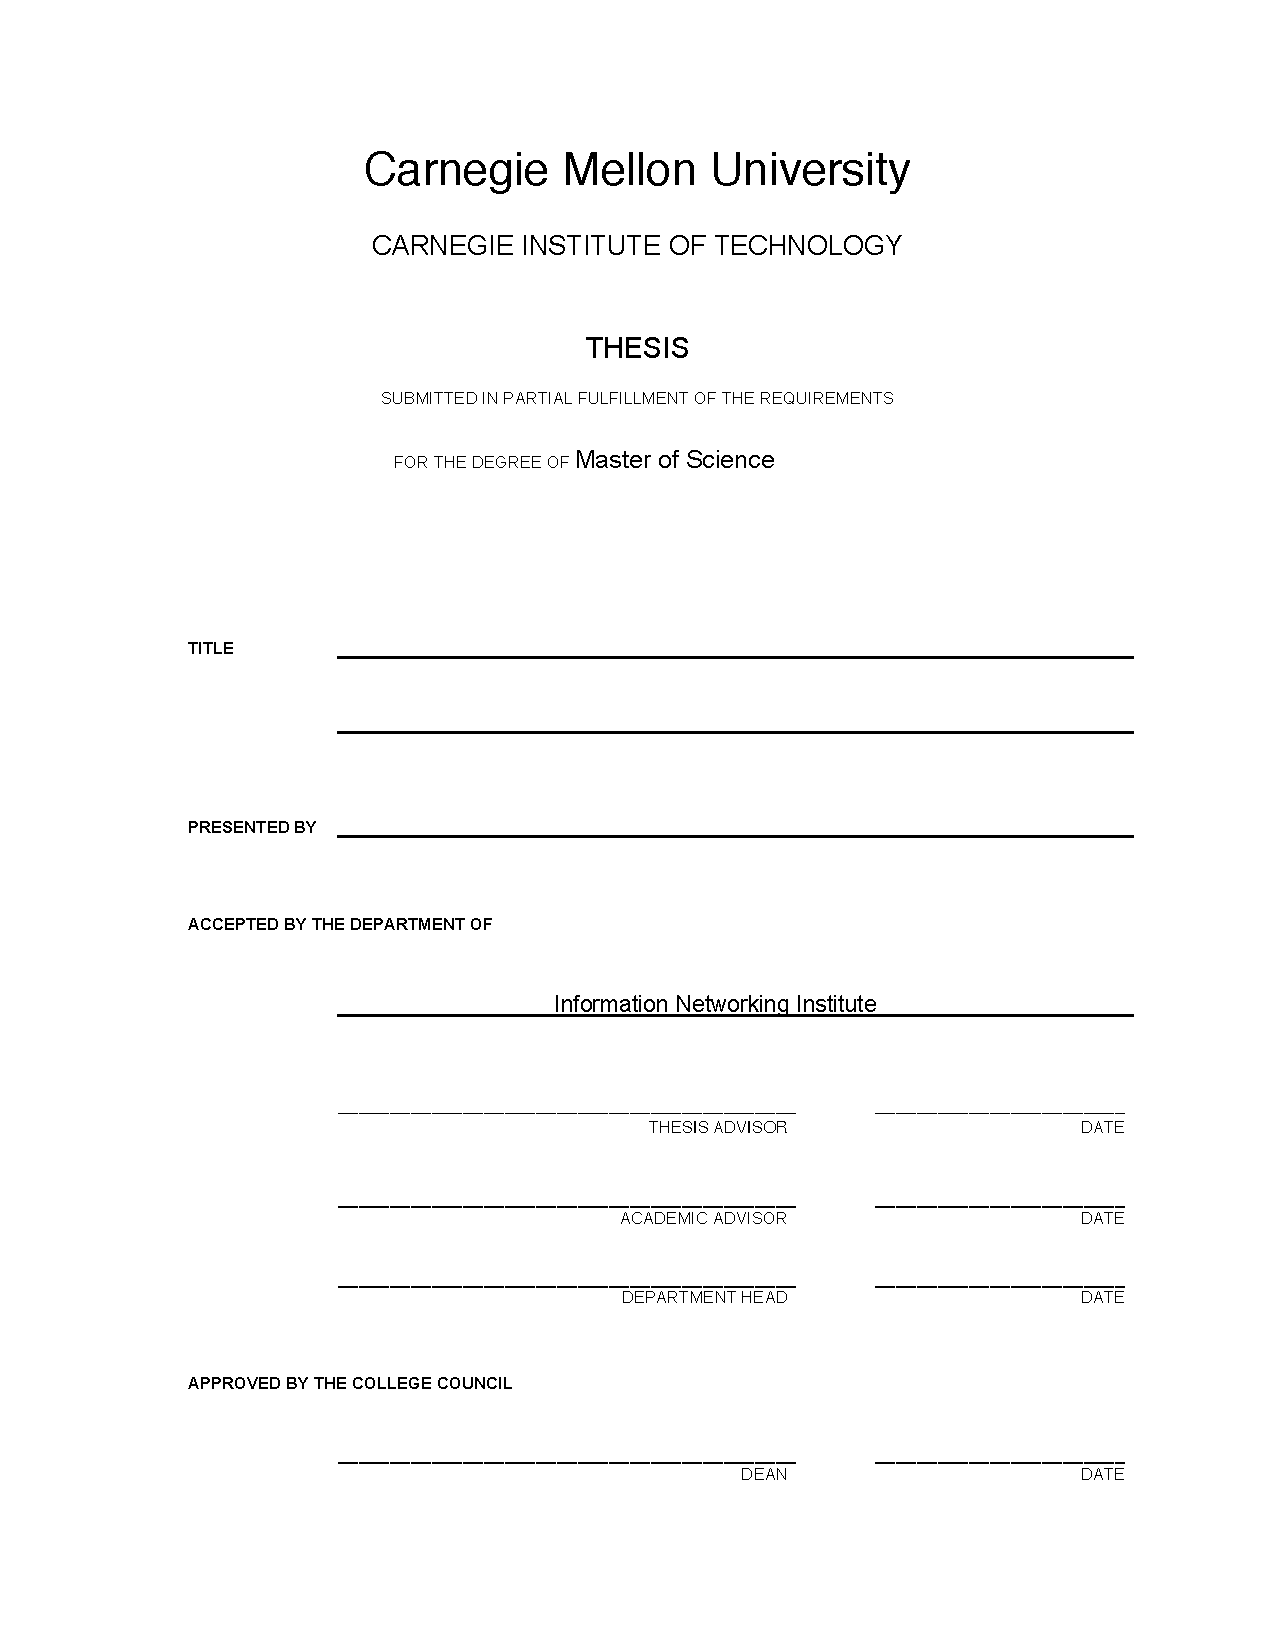
\includepdf[pages={1}]{signature.pdf}

%-----------------------------------------------------------------------------%
% TITLE PAGE -- provides UMI abstract title page & copyright if appropriate
%-----------------------------------------------------------------------------%
\maketitle

%-----------------------------------------------------------------------------%
% ACKNOWLEDGEMENTS -- included file should start with '\acknowledgements'
%-----------------------------------------------------------------------------%
\acknowledgements

\setcounter{page}{2}

Thank you to Maverick Woo who initially proposed the idea for this thesis and has guided me throughout this journey. I would also like to thank Patrick Tague for helping me through major milestones throughout this project and providing useful feedback when requested. Thank you to the Scholarship for Service program for funding my time at Carnegie Mellon and this thesis. Finally, I am forever grateful for the invaluable support my family and friends have provided me, without which none of this would be possible.}

%-----------------------------------------------------------------------------%
% ABSTRACT -- included file should start with '\abstract'.
%-----------------------------------------------------------------------------%
\abstract

Write your abstract here.  You should not include references or mathematical notation.}

%-----------------------------------------------------------------------------%
% FRONTMATTER -- ToC is required, LoT and LoF are required if you have any
% tables or figures, respectively. List of Abbreviations and Symbols is 
% optional.
%-----------------------------------------------------------------------------%
\tableofcontents % Automatically generated
\newpage
\listoftables	% If you have any tables, automatically generated
\addcontentsline{toc}{chapter}{List of Tables}%
\newpage
\listoffigures	% If you have any figures, automatically generated
\addcontentsline{toc}{chapter}{List of Figures}%
\newpage
%\abbreviations

% You can put here what you like, but here's an example
%Note the use of starred section commands here to produce proper division
%headers without bad '0.1' numbers or entries into the Table of Contents.
%Using the {\verb \begin{symbollist} } environment ensures that entries are
%properly spaced.

\section*{Symbols}

Put general notes about symbol usage in text here.  Notice this text is
double-spaced, as required.

\begin{symbollist}
	\item[$\mathbb{X}$] A blackboard bold $X$.  Neat.
	% Optional item argument makes the symbol/abbr
	\item[$\mathcal{X}$] A caligraphic $X$.  Neat.
	\item[$\mathfrak{X}$] A fraktur $X$.  Neat.
	\item[$\mathbf{X}$] A boldface $X$.
	\item[$\mathsf{X}$] A sans-serif $X$. Bad notation.
	\item[$\mathrm{X}$] A roman $X$.
\end{symbollist}

\section*{Abbreviations}

Long lines in the \texttt{symbollist} environment are single spaced, like in
the other front matter tables.

\begin{symbollist}
	\item[AR] Aqua Regia, also known as hydrocloric acid plus a splash of 
	nitric acid.
	\item[SHORT] Notice the change in alignment caused by the label width
	between this list and the one above.  Also notice that this multiline
	description is properly spaced. 
	\item[OMFGTXTMSG4ME] Abbreviations/Symbols in the item are limited to
	about a quarter of the textwidth, so don't pack too much in there.
	You'll bust the margins and it looks really bad.
\end{symbollist}
} % List of Abbreviations. Start file with '\abbreviations'

%==============================================================================
%-----------------------------------------------------------------------------%
%
% MAIN BODY OF PAPER
%
%
%-----------------------------------------------------------------------------%
\chapter{Introduction}
\label{sec:intro}

This thesis would like to explore the idea of using automated techniques for modernizing old C codebases. C standards are published every so often, and can include a number of useful additions that developers may want to take advantage of. This may be the case for C's new checked arithmetic macros. These macros are designed to perform and check arithmetic operations so that bugs related to integer safety are caught and handled at runtime.

The main issue faced by a lot of developers in the real world is that it may take a long time to actually rewrite their codebases to utilize, say, checked arithmetic macros. Modernizing codebases is often plagued by this issue, which may motivate developers to just rewrite their codebases completely. Doing a complete rewrite, especially in a more modern language, has a lot of benefits. However, doing this is just not practical and often misguided. Specifically with integer arithmetic, overflows and wraparounds still occur in modern languages. Thus, it may be more beneficial to perform an automatic rewrite that uses these macros before incurring the cost of a completely new implementation.

It is in the interest of both these developers and society as a whole to adopt features, especially ones that make code more secure. This is the justification for this thesis, which aims at finding a method for automatically modernizing codebases to use checked arithmetic. Due to the nature of these new macros, a number of challenges need to be overcome to actually be successful.

The main issue related to rewriting statements is the issue of intermediate types. When an arithmetic expression is written, the programmer must use intermediate variables to store and check for overflow. This is simply due to the construction of these macros. Because integer overflow and wraparound depend on the width of the variables involved, selecting the right types of the intermediate variables is imperative to successfully rewriting these statements correctly. Another issue is related to how the macros only operate on a subset of the integer types and operations. Thus, not all operations that can overflow can be rewritten using the checked arithmetic macros.

Finding an automatic method for rewriting statements that tackles these main issues will open the door for developers to harness these new language features until more robust solutions are presented to them in the future.}
%\chapter{Background}
\label{sec:background}

This chapter will explore the background required to fully understand the motivation of this thesis, the current landscape with regard to integer safety, and important details related to the macros introduced in the new C23 standard. It will cover a short history of C and the C standard to provide the reader with some context on the philosophies of C and how new language features are introduced. This will be followed by a discussion on the development pipeline for safety critical systems, which will also be useful for understanding the requirements of the problem space. The next section will cover integer safety. These sections will further describe the problem space of this thesis. Following this description will be a taxonomy of approaches and their relative effectiveness. The chapter will conclude with relevant details of the new C23 standard that motivated this particular project.

\section{C and the C Standard}

C is a general-purpose imperative procedural compiled programming language. It features important tools like a static type system, raw memory manipulation, portable code generation, and a lightweight runtime.

C as a programming language was initially developed by Dennis Ritchie in the early 1970's at Bell Labs \cite{ritchie}. The purpose of the language was to provide a higher-level programming interface to build operating systems like Unix. C was first standardized in 1989 by the American National Standards Institute (ANSI) and later standardized by the International Organization for Standardization (ISO) in 1990 \cite{ansi}\cite{ISO}. Since then, several more standards have been released to add or remove features from the official language standard. The process of creating a new C standard follows the general ISO standardization process which starts with a proposal, and ends with a publication stage. During this process, there are a series of meetings between stakeholders including the official C standards committee (WG14)\cite{wg14}. The C standards committee is an international group of experts tasked with maintaining, updating, and refining the C standard.

\subsection{Unspecified Behavior and Undefined Behavior}
The C language specification categorizes the behaviors of programs generated by a C compiler. There are some behaviors, however, that are not explicitly defined by the standard. These include \textit{undefined behavior}, \textit{unspecified behavior}, \textit{implementation-defined behavior}, and \textit{locale-specific behavior} \cite{c_standard}. The two behaviors relevant to this thesis are undefined and unspecified behavior.

Undefined behavior occurs when a program is not well formed and exhibits some statement that is ``undefined'' \cite{c_standard}. This can include out of bound accesses, null pointer dereferences, and signed integer overflow. When such a statement is written, the standard allows the compiler to do anything it wants (including making demons shoot out of your nose \cite{nasal_demons}). These statements are often a source of optimization, but can also result in security vulnerabilities.

Unspecified behavior are related to statements that can have multiple outcomes the compiler does not need to document. An example of this is the order of evaluation: a statement with multiple subexpressions does not have to be evaluated in specific or consistent order. This allows compilers again to optimize their instructions to maximize performance.

\section{The Development of Safety Critical Systems}

In many cases, it is unacceptable to have a software fault. This would be the case for many safety critical systems like locomotives, aircraft, cars, or power plants, to name a few. It may not be possible to completely eliminate all bugs, however the software development pipelines for these systems is designed to catch and fix bugs as early as possible. There are several regulatory standards imposed on different systems, and we will not be going over all of them. However, it is important to note a common technique that is commonly employed: manual code review \cite{faa}\cite{do}. That is, when code is written, other developers will need to manually certify that the newly written code does not contain some set of bugs defined in a standard checklist. This will be an important detail as some approaches to code modernization will not take place at the source level, which will need to be reviewed by humans before being certified. 

\section{Integer Safety}

The topic of integer safety has a long and interesting history involving a number of different systems. In this section we will discuss that integer safety is, how violations of integer safety occur, and some real world examples of bugs caused by integer overflow.

\subsection{Integer Representation}

When a integer is declared and initialized, it's underlying value will be represented by a collection of bits. The C standard defines a number of different integer types and can be broken into two different categories: unsigned and signed integers. Unsigned integers represent numbers using raw binary numbers ranging from 0 to $2^{\text{width}(\text{type})} - 1$ where $width(type)$ is the number of bits that represent the type of the integer. Standard unsigned integer types and their widths on x86-64 using the LP64 model include \texttt{unsigned char} (8 bits), \texttt{unsigned short int} (16 bits), \texttt{unsigned int} (32 bits), \texttt{unsigned long int} (64 bits), \texttt{unsigned long long int} (64 bits) \cite{LP64}.

Signed integers are meant to store positive and negative numbers, something you cannot do using an unsigned integer. Standard signed integer types and their widths on x86-64 using the LP64 model include \texttt{signed char} (8 bits), \texttt{short int} (16 bits), \texttt{int} (32 bits), \texttt{long int} (64 bits), \texttt{long long int} (64 bits). The C standard also allows compilers to represent signed integers in three different ways: sign and magnitude, one's complement, and two's complement \cite{c_standard}. Virtually all modern compilers will represent signed integers using two's complement, so only the implications of this representation will be discussed. Two's complement works by treating the most significant bit as a \textit{sign bit}, then giving it a weight of $-2^{N - 1}$ when calculating the decimal value of each bit. Two's complement is the most popular representation of integers because of properties it has to make arithmetic operations easy and does not have issues like a positive and negative 0 representation like one's complement. One important detail however, is the most negative value that two's complement cannot be represented as a positive number using the same number of bits due to the asymmetry of two's complement.

With any type of integer in C, they are represented using a finite set of bits. This means that depending on the number of bits available for a particular integer type, there is a finite set of numbers that can be represented. This leads to the question: what happens when I try to store an integer that needs more bits than is available in a particular type? The answer is truncation, which can result in a misinterpretation of the newly assigned value. The specifics on how the compiler will react to such a situation will depend on the types involved.

When a value that is too large for an \textit{unsigned integer} is stored, \textit{wraparound} occurs. Given an unsigned integer of width 16, only the 16 least significant bits of the value will be stored in the unsigned integer. A property of binary representation is this operation becomes a modulus operation, meaning any value placed in an unsigned destination will have the value $n \bmod width(type)$, where $n$ is the value to place in the unsigned integer and $type$ is the unsigned integer type of the destination.

Interestingly, this behavior is considered defined behavior in the C language specification \cite{c_standard}. This is a point of controversy within the C community but the rational is because representation itself is always a modulus operation, something that some programmers take advantage of, the concept of an \textit{overflow} in an unsigned type has no meaning. Furthermore, this behavior is closer to how hardware would perform, wrapping around when the maximum or minimum value is reached.

\subsection{Integer Overflow}

An \textit{integer overflow} occurs when an operation involving a \textit{signed integer} results in a value that is too large or small to be represented in the resultant type. The C standard considers integer overflow undefined behavior, which has a number of implications as mentioned earlier in this chapter. Operations that can cause overflow are listed in table 2.1.
\begin{table}[h!]
\centering
\begin{tabular}{|c|l|}
\hline
\textbf{Operator} & \textbf{Description} \\
\hline
\texttt{+}        & Addition \\
\texttt{-}        & Subtraction \\
\texttt{*}        & Multiplication \\
\texttt{/}        & Division \\
\texttt{\%}       & Modulo \\
\texttt{<<}       & Left shift\\
\hline
\texttt{+=}       & Compound addition assignment \\
\texttt{-=}       & Compound subtraction assignment \\
\texttt{*=}       & Compound multiplication assignment \\
\texttt{/=}       & Compound division assignment \\
\texttt{\%=}      & Compound modulo assignment \\
\texttt{<<=}      & Compound left shift assignment \\
\hline
\texttt{++}       & Pre/post-increment \\
\texttt{--}       & Pre/post-decrement \\
\hline
\end{tabular}
\caption{Operations that can Overflow}
\end{table}

Something interesting to note is that division and modulo operations can overflow. This is due to the asymmetry of two's complement as previously mentioned, where the most negative value of two's complement cannot be represented as a positive number. Thus, any operation that can switch the sign (like division and modulo) on the smallest possible value will result in an overflow. Because this overflow depends on the way integers are represented, technically this subset of operations become safe when a different representation is used, like one's complement.

\subsection{Integer Conversion}

Integers can be converted from one integer type to another explicitly through a type cast, or implicitly within a mixed-typed statement. For example, an implicit cast could be inserted by the compiler in an arithmetic expression, an assignment, or even a function call. The intention of these rules is to make it easy for programmers to write mixed-typed statements without having to worry about explicit casts, so long as they remember the rules that govern them.

There are three concepts that are outlined in the C standard regarding integer conversions: \textit{integer conversion rank}, \textit{integer promotion}, \textit{usual arithmetic conversions} and \textit{default arithmetic conversions}. These concepts are explained in the following subsections:

\subsubsection{Integer Conversion Rank}

Each integer type is assigned a type of \textit{rank} that is used to govern how conversions are made between different types. The rank assigned to a type is determined by the rules in Table 2.2 \cite{c_standard}.

\begin{table}[h!]
\centering
\begin{tabular}{|c|p{13cm}|}
\hline
\textbf{Rule} & \textbf{Description} \\
\hline
1 & The ranks of all signed integer types are different and increase with their precision.\\
\hline
2 & The ranks of all signed integer types equal the ranks of the corresponding unsigned integer types. \\
\hline
3 & The rank of any standard integer type is greater than the rank of any extended integer type or bit-precise integer type of the same size.\\
\hline
4 & The rank of \texttt{char} equals the rank of \texttt{signed char} and the rank of \texttt{unsigned char}. \\
\hline
5 & The rank of \texttt{bool} is less than the rank of any other standard integer type. \\
\hline
6 & The rank of any enumerated type equals the rank of its compatible integer type. \\
\hline
7 & Ranking is transitive.\\
\hline
8 & The rank of a bit-precise signed integer type shall be greater than the rank of any standard integer type with less width or any bit-precise integer type with less width. \\
\hline
9 & The rank of any bit-precise integer type relative to an extended integer type of the same width is implementation-defined. \\
\hline
10 & Any aspects of relative ranking of extended integer types not covered above are implementation-defined. \\
\hline
\end{tabular}
\caption{C23 Integer Conversion Rank Rules}
\end{table}

The purpose of these rules becomes clear in the next section.

\newpage
\begin{table}[h!]
\centering
\begin{tabular}{|p{4cm}|p{10cm}|}
\hline
\textbf{Condition} & \textbf{Conversion Rule} \\
\hline
Target type can represent the value & The value is unchanged. \\
\hline
Target type is \texttt{unsigned} and cannot represent the value & The value $2^b$, where $b$ is the number of value bits in the target type, is repeatedly added or subtracted to bring the value into range. In other words, unsigned integers implement modulo arithmetic. \\
\hline
Target type is \texttt{signed} and cannot represent the value & The result is implementation-defined behavior (which may include raising a signal). \\
\hline
\end{tabular}
\caption{Integer Conversion Rules in C23}
\end{table}
\newpage

\subsubsection{Integer Promotion}

Integer promotion is the implicit conversion of any type with a rank less than an \texttt{int} or \texttt{bool} to an \texttt{int}. Note that the promoted type can be signed or unsigned. Furthermore, these promotions are intended to preserve the value and sign of the initial value. The rules that determine how promotion is handled can be found in Table 2.3.

Integer promotion only apply to the following:
\begin{itemize}
    \item Usual arithmetic conversions
    \item Default argument promotions
    \item Operands of the \texttt{++} and \texttt{--} operators
    \item Operand of the \texttt{\textasciitilde} operator
    \item Both operands of the \texttt{<<} and \texttt{>>} operators
\end{itemize}

The next section will cover the case most relevant to this project, usual arithmetic conversions.

\subsubsection{Usual Arithmetic Conversions and Default Argument Promotions}

When a mix-typed statement is written, the compiler will need to calculate the \textit{common real type} of the operation itself, which will be used to complete the operation. Operations that would trigger a conversion include binary arithmetic, relational operations, bitwise operations, and the conditional operator. The rules for how the common real type is generated can be found in appendix \ref{appendix:common_real_type}.


As mentioned in the integer promotion subsection, default argument promotions can also trigger integer promotion. This occurs when the arguments are passed to a variadic function and are matched to the ellipsis parameter.

Now will these concepts explained, it is important to understand how these rules can be a source of error. The implication is that these casts can result in a loss of value (i.e. conversion where the magnitude of original value cannot be preserved) or a loss of sign (i.e. converting from a signed value to an unsigned value will mean negative values are no longer represented).

Consider the following example \cite{secure_coding} :

\begin{center}
\parbox{0.9\linewidth}{
\texttt{unsigned int ui = ULONG\_MAX;\\
signed char c = -1;\\
if (c == ui) \{\\
\hspace*{2em}puts("Why is -1 = 4,294,967,295???");\\
\}
}}
\end{center}

In the code above, the signed char \texttt{c} is compared to signed int \texttt{ui}. As a result, \texttt{c} is promoted to an \texttt{unsigned int} and now represents a very large unsigned value.

\subsection{Case Studies}

There have been a number of real-world bugs that have been caused by integer overflow and wraparound. One of the most famous examples is the Ariane 5 rocket disaster. The disaster was caused by an integer overflow that resulted erroneous horizontal velocity values, leading to the rocket to self-destruct \cite{a5}. The damage exceeded \$370 million dollars \cite{a5_cost}.

Another prominent example was the Therac-25 radiation therapy machine. This machine was meant to deliver a dosage of radiation to patients to treat illnesses like cancer. However, there were a number of software related issues including an arithmetic overflow that caused certain safety checks to be bypassed \cite{therac}. The result of these errors resulted in radiation doses that exceeded 100 times the intended amount in a smaller area. Patients developed radiation burns and three individuals lost their lives.

One thing to note is this issue is not constrained to C. The overflow in the Ariane 5 was in Ada. In all, these examples should demonstrate the consequences of poor integer safety.

\section{Previous Approaches to Ensuring Integer Safety}

Given how long integer safety has been an issue for C programmers, there are a number of approaches that have been adopted by the community. They each have pros and cons and are discussed in the following subsections. Note that from this point on we only consider approaches to integer safety that do not involve arbitrary precision types.

\subsection{General Approaches for Detecting Overflow and Wraparound}

There are a number of general approaches that can be used to detect when overflow or wraparound occurs that involve modifying or instrumenting code to catch these cases. These approaches don't depend on any particular build system or language as they are implemented by the programmer manually. These are discussed below:

\subsubsection{Pre and post condition testing}
The most basic approach to detecting overflow and wraparound involve introducing checks before and after the risky operation. For example, take the following operation:

\begin{center}
\parbox{0.9\linewidth}{
\texttt{int a, b, c;\\
// initialize a and b\\
c = a + b;}
}
\end{center}

The line \texttt{c = a + b} may overflow. Using a precondition check, we can test if the current values of \texttt{a} and \texttt{b} will indeed trigger an overflow before performing the operation. This could be written like so \cite{secure_coding}:

\begin{center}
\parbox{0.9\linewidth}{
\texttt{int a, b, c;\\
// initialize a and b\\
if ((b > 0 \&\& a > INT\_MAX - b) ||\\
\hspace*{2em}(b < 0 \&\& a < INT\_MIN - b)) \{\\
\hspace*{1.5em}// OVERFLOW\\
\} else \{\\
\hspace*{1.5em}c = a + b;\\
\}}
}
\end{center}
In english, the code above will test that there is room between the current value of \texttt{a} and the upper and lower bounds of signed integer representation.

There is a notion of a post-condition test as well. Below is an example of how one would right a post-condition check for wraparound for two unsigned integers:

\begin{center}
\parbox{0.9\linewidth}{
\texttt{unsigned a, b, c;\\
// initialize a and b\\
c = a + b;\\
if (c < a) \{\\
\hspace*{1.5em}// WRAPAROUND\\
\}}
}
\end{center}

Although easy to implement, there are a number of issues with this approach. One is related to performance: constantly checking for overflow can introduce overhead and damage performance. Another is it becomes difficult to write multi-operation arithmetic statements like \texttt{int c = a + b + c}, which would need to perform two operations and thus two checks. Although this is a simple example, these statements can get quite complex and difficult to rewrite. This issue is further complicated by the fact that the order of evaluation is unspecified behavior and may vary between different compilers.

\subsubsection{Using Status Flags}

In x86, there exist instructions that will perform a type of postcondition check for overflow once an operation is performed. The overflow (\texttt{OF}) and carry (\texttt{CF}) flags will be set after an instructions like \texttt{add}, \texttt{sub}, and \texttt{mul} if overflow or wraparound occurs \cite{x86}. Instructions like \texttt{jo} and \texttt{jc} can then perform jumps if these bits are set to an overflow or wraparound handler.

This approach also introduces overhead similar to the general checks previously mentioned. The performance issue is actually worse in this case, since the compiler likely won't be able to optimize this assembly. Furthermore, this approach is not portable and depends on both the architecture of the system and the compiler extensions supported to write inline assembly (the most likely approach to injecting these instructions). It again suffers from issue of potentially writing overly complex statements to check multi-operation statements.

\subsubsection{Casting the result to a larger type}

A simple solution to detecting overflow and wraparound in addition and multiplication is to first cast the operands to a larger type, perform the operation and check for overflow, then downcast to the original resultant type. For addition, any result can be represented by $w+1$ bits, where $w$ is the width of the largest operand. This rule is the same for multiplication, however each operand needs to be at least $2w+1$.

Once the operation is complete, the result can then be range checked in a type of postcondition check, then downcasted to the intended type if no overflow or wraparound occurred. This approach is simple however it does depend on the compiler since C does not guarantee any standard type is larger than any other standard type.

\subsection{Language-based Approaches}

C is a very old language and its ability to produce integer arithmetic errors largely stems from this fact. Since C was created, many other languages have been developed and have addressed the issue of integer safety in different ways. The following are several notable examples.

\subsection{Python}

Python was initially created as a learning language by Guido van Rossum in 1991 as a type of learning language. It is a dynamically typed, mutli-paradigm scripting language. In Python, integers are represented using arbitrary precision, meaning integers can have as many bits as they need to be represented granted there is enough memory on the system \cite{python_types}. As a result, for integer types there is no notion of an ``overflow" or ``wraparound".

Interestingly, there is still an \texttt{OverflowError} exception that can be raised if an integer is too large to be represented \cite{python_overflow}. This error cannot occur for integers however, and instead a \texttt{MemoryError} is raised. According to the documentation it may still be raised if an integer is outside some range due to historical reasons. For completeness, floating-point operations \textit{can} overflow, which is due to a lack of standardization for handling floating-point exceptions in C.

\subsubsection{Java}

Integers are represented in Java using two's complement arithmetic and will wraparound when a value is too large to be represent a particular value \cite{java_int}. To address this, Java 8 provides a set of functions that can perform operations and either return the result of the operation or throw an exception. These functions are: \texttt{addExact}, \texttt{subtractExact}, \texttt{multiplyExact}, \texttt{incrementExact}, \texttt{decrementExact}, and \texttt{negateExact} \cite{java_exact}.

Another option that Java provides is the \texttt{BigInteger} type, which allows for arbitrary precision integers \cite{bigint}.

\subsubsection{Rust}

Rust is often used as a modern replacement for C and C++ given it's capability as a systems programming language while still supporting many safety mechanisms. Of these features is integer safety. When a Rust program is compiled in debug mode, checks are inserted in the binary to detect integer overflow \cite{rust_book}. When an overflow is detected, a \textit{panic} is triggered. An important detail here is that these checks are removed when a rust binary is compiled in \textit{release} mode. To address this, Rust provides a set of \texttt{checked*} functions to detect integer overflow due to arithmetic operations \cite{rust_checked}. These will ensure that checks are performed even in release builds. Downsides of this approach are rewrites of complex operations can be tricky and there is a performance overhead.

Perhaps the most dangerous aspect of this is what most developers think Rust is capable of. Namely, that as long as the \texttt{unsafe} keyword is not being used, integer overflow is not something to worry about. This is simply not the case, as integer safety is still an issue in release builds.

\subsection{Checked Arithmetic Libraries}

Another approach to making C arithmetic safe is to use an external library to perform arithmetic in a safe manner. The exact approach for how code should be written or rewritten will depend on the library, and can also issues related to compatibility. The following subsections cover some modern safe arithmetic libraries for C and C++.

\subsubsection{SafeInt}

The SafeInt library approaches integer safety by providing functions to explicitly cast integers and perform arithmetic operations. This is a great approach since these are the sources of integer errors. In effect this library provides safe functions for assignment, casting, comparison, arithmetic, and logical operations. Below is an example given in their documentation:

\begin{flushleft}
\begin{minipage}{\linewidth}
\texttt{int main()\\
\{\\
\hspace*{1.5em}int divisor = 3;\\
\hspace*{1.5em}int dividend = 6;\\
\hspace*{1.5em}int result;\\
\hspace*{1.5em}bool success = SafeDivide(dividend, divisor, result);\\
\hspace*{1.5em}success = SafeDivide(dividend, 0, result);\\
\}
}
\end{minipage}
\end{flushleft}


This library was originally written for C++, however now supports C via the \texttt{safe\_math.h} and \texttt{safe\_math\_impl.h} header files.

\subsubsection{Intel Safe Arithmetic}

The Intel Safe Arithmetic library approaches the issue of integer safety via compile-time checks. It provides safe versions of common types, putting them in a type of ``safe arithmetic environment". This means any operations performed on these new types are checked for unsafe behavior including signed overflow and unsigned wraparound.

This approach has a massive benefit: there is no runtime overhead. Since these checks are performed at compile-time and any potential errors generate warnings, no instrumentation or handling needs to be inserted to detect and handle overflows. Furthermore, so long as the types are changed existing code can remain relatively similar and reap the benefits of integer safety. The downside to this library is it only supports C++.

\subsubsection{safe\_numerics}

The safe\_numerics library uses a hybrid compile and runtime approach. Similar to Intel's Safe Arithmetic library, new safe types are provided that can be used like any other builtin type. When enough information can be determined that an overflow may occur at compile-time, a warning is generated. If not, and an overflow occurs during runtime, the overflow is handled via runtime exception that the developer can handle. This has the added benefit of being more complete than only using a compile-time approach, however there is a small runtime overhead due to the added runtime checks. This library is also only written for C++.

\subsection{Compiler-based Approaches}

Compiler engineers have developed techniques to automatically mitigate integer overflow and wraparound vulnerabilities. These include inserting instrumentation when an overflow is detected and providing functions for developers to easily perform precondition tests.

\subsubsection{The \texttt{-ftrapv} flag}

Compilers like GCC and Clang provide a number of compiler flags that instruct the compiler on how to deal with integer overflow and wraparound. The \texttt{-ftrapv} flag will instruct the compiler to insert instrumentation to detect and handle signed integer overflow \cite{ftrapv}.

The downsides of this approach is there is again an overhead to inserting these checks and this flag is known for having some implementation issues. These issues include the conditional branches used to handle the trap (which can be expensive) and will only detect overflow for a subset of operations that can produce an overflow. Another is this flag will not detect unsigned wraparound, which may be unintended behavior.

Furthermore, this approach also has the limitation of not inserting changes at the source level. This could be an issue for development pipelines that need to verify changes made by any automatic tools including passes by a compiler like a safety critical system.

One interesting note is that GCC seems to implement handling by calling \texttt{abort()}, which is not always the correct approach to handling overflow or any kind of error. Clang however does have a \texttt{-ftrapv-handler} flag that allows developers to specify a function to call when an error is detected \cite{clang-ftrapv}.

\subsubsection{Undefined Behavior and Integer Overflow Sanitizers}

Both GCC and Clang provide an Undefined Behavior Sanitizer (UBSan), which will instrument the compiled binary to detect a number of undefined behaviors in a program \cite{gcc-ubsan}\cite{clang-ubsan}. This is similar to using the \texttt{-ftrapv} flag but spans a number of other patterns that can result in undefined behavior. This includes, out-of-bounds array subscripts, bitwize shifts that are too large, null-pointer dereferences, and signed integer overflow.

UBSan is slightly better than using the \texttt{-ftrapv} flag since it can also be configured to check for unsigned integer overflow. Besides this benefit, this approach suffers from the same issues using \texttt{-ftrapv} incurs.

\subsubsection{Overflow Checking Functions}

GCC and Clang offer language extensions for checking if an arithmetic operation will overflow\cite{gcc-lang-ext}\cite{clang-lang-ext}. The general structure of these functions are to pass both arguments and the destination for the operation to one of these functions. This function will then both perform the operation and check for overflow using the promoted operands. It will then return 1 if an overflow is detected and 0 otherwise. The programmer is meant to check the return value of this operation then handle the case where an overflow is detected.

For the sake of space, only a subset of Clang's extensions are listed below:
\begin{tabbing}
\texttt{bool \_\_builtin\_add\_overflow(type1 x, type2 y, type3 *sum);}\\
\texttt{bool \_\_builtin\_sub\_overflow(type1 x, type2 y, type3 *diff);}\\
\texttt{bool \_\_builtin\_mul\_overflow(type1 x, type2 y, type3 *prod);}
\end{tabbing}

With regards to making source-level checks to detect integer overflow, this is the best approach. There are still downsides around readability and ensuring programmers call these functions and handle errors correctly, which are shared with issues pre and post condition checks have. Furthermore, these are compiler \textit{extensions}, and are not part of the C standard. This means there is a dependence on both compiler support and how the compiler implements these functions (the names and signatures of these functions are very different between Clang and GCC).

Notably, both GCC and Clang offer signed and unsigned versions of these functions, and implement the generic check function (i.e. \texttt{builtin\_add\_overflow(type1 x, type2, type3, *sum)} such that it will detect both signed integer overflow and unsigned integer wraparound.

\subsection{Testing and Analysis}

Software testing and using automated or manual analysis is likely the most common approach to avoiding integer arithmetic errors. These techniques can range from simple unit tests to complex guided fuzzing or even formal verification. Because the range of approaches is quite wide and the pros and cons of this approach really depend on the technique applied here. The approaches we will consider are static analysis, testing, and manual review.

Static analysis tools can be quite powerful and will generally involve running the tool, then rewriting code to prevent or remove a line of source that could be unsafe \cite{secure_coding}. The benefit is that these tools can integrate nicely in a development environment, however the main downside will be false positives and negatives. Static analysis tools are generally more prone to producing false positives. When the number of false positives is reduced, this may also result in false negatives. It is very difficult to build a static analysis tool that is both sound and complete, so developers should not rely solely on this approach.

Testing is a good practice for any software development, and can quickly locate bugs before they become bigger issues. Unfortunately, this approach cannot make guarantees about how code will behave in the field and it is difficult to ensure all possible inputs are tested.

Finally, the last approach we will consider is a manual source code audit. This is also common practice, and can be quite effective for locating bugs. However this approach may fail to locate bugs due to the error-prone humans it relies on.

The biggest downside to all of these approaches are how much more involved humans must be, which suffers from issues related to human error and the cost of labor.

\section{The C23 Approach}

In December 2023, the C23 standard was officially published \cite{c_standard}. Among the changes to the C standard was a set of checked arithmetic functions for testing if certain operations would overflow \cite{ckd_arith}. These functions were essentially inspired by the language extensions GCC and Clang have for detecting integer overflow and wraparound. As a result, the GCC and Clang compilers have essentially just provided implementations that wrap their existing extensions.

\subsection{The ckd\_add, ckd\_sub, and ckd\_mul Macros}

C23 defines the set of checked arithmetic macros in the \texttt{<stdckdint.h>} as follows:

\begin{flushleft}
\texttt{bool ckd\_add(type1* result, type2 a, type3 b);}\\
\texttt{bool ckd\_sub(type1* result, type2 a, type3 b);}\\
\texttt{bool ckd\_mul(type1* result, type2 a, type3 b);}
\end{flushleft}

Each function will perform the operation as if an infinite-precision model is being used, then return \texttt{1} if an overflow occurs. Note that these are ``type-generic" macros and can take several types. The standard says that ``\texttt{type2} and \texttt{type3} shall be any integer type other than ``plain” \texttt{char}, \texttt{bool}, a bit-precise integer type, or an enumerated type, and they need not be the same. \texttt{*result} shall be a modifiable lvalue of any integer type other than ``plain” \texttt{char}, \texttt{bool}, a bit-precise integer type, or an enumerated type" \cite{ckd_arith}.

\subsection{Open Questions}

These macros are a welcome addition to the C programming language and hopefully will be used to ensure critical operations are checked. However, there are still some open questions about this approach, which are discussed below:

\subsubsection{Should these functions work for signed and unsigned types?}
As we have seen in the language extensions provided by GCC and Clang, signed and unsigned macros have been provided to be specific with the type of behavior that is being detected. So far there is no distinction here in the C23 standard, and the standard does not discuss this detail. Tests have revealed that these macros do detect unsigned wraparound, however this is likely implementation defined behavior and could result in issues if different compilers are used.

\subsubsection{How do you ensure the correct types are used?}

The type of the destination and operands are very important for determining if an operation will result in an overflow or wraparound. Furthermore, C has a number of complex rules that govern implicit casts as mentioned previously. The concern here is should the resultant type be determined exclusively by the developer? If not, could the compiler be used to determine if there is going to be an overflow?

\subsubsection{How is a two argument signature going to change things?}

There is a proposal to move from a three argument macro to a two argument macro that just contains the operands of an argument. This is supposedly a future plan but can also suffer from a similar issue to the typing issue: how will the compiler determine the resultant type and thus correctly detect overflow?

\subsubsection{What about other operations and types?}

A final question is how will these macros evolve to detect overflow in other operations. The restrictions the C23 standard places on the types of the destination and operands is quite limiting, and makes these macros ineffective against a very large proportion of operations that may overflow.} % A regular chapter, starts with '\chapter{Title}'
\chapter{Nonsense text for layout proofing}
\label{hello}

Enjoy some Lorem Ipsum text!
This should create about two full pages of text so you can verify the
margins are correct (especially if you're doing two-sided).

\section{Lorem Ipsum}
Lorem ipsum dolor sit amet, consectetuer adipiscing elit. Sed vitae leo.
Pellentesque quis nisi id orci consectetuer posuere. Quisque malesuada
rhoncus dui. Vivamus mi. Mauris commodo. Phasellus lacus magna, feugiat ac,
blandit ut, rutrum id, massa. In consectetuer magna vel justo. Cras eu
diam. Nullam tortor turpis, bibendum non, consequat ac, tincidunt non,
nisi. 

Curabitur sagittis dignissim arcu. Pellentesque habitant morbi
tristique senectus et netus et malesuada fames ac turpis egestas.
Vestibulum ullamcorper. Curabitur faucibus euismod nulla. Vivamus sagittis.
Sed fermentum neque a risus vestibulum convallis. Morbi id massa ut arcu
mollis commodo. Aliquam erat volutpat.  Pellentesque fringilla pellentesque
nisi. Morbi tristique ornare libero. Vestibulum turpis sapien, iaculis ut,
cursus non, condimentum in, tortor. Aenean vehicula. Integer egestas
tincidunt erat. Aenean euismod ante vel lectus. Duis ac sapien vel erat
euismod aliquet. Vivamus tempor placerat nibh. Curabitur pharetra, orci
consequat pulvinar ultricies, orci enim tempor augue, non lacinia orci nisl
et nibh. Nunc gravida dictum turpis.  Duis sollicitudin commodo massa. Nam
ac nunc. Fusce sodales posuere velit. Nunc ullamcorper sodales urna. Donec
consectetuer accumsan ante. Morbi feugiat rutrum mauris. Praesent malesuada
auctor est. Pellentesque quis odio non nulla ornare imperdiet. Aliquam
dapibus. Suspendisse posuere, magna in molestie varius, ipsum velit rhoncus
nisi, nec bibendum pede mauris in urna. Morbi purus lectus, molestie quis,
laoreet id, tincidunt at, ligula. 

Praesent sit amet libero id arcu
adipiscing tristique. Quisque libero erat, bibendum nec, malesuada in,
gravida et, urna. Phasellus molestie vulputate nisi. Nullam massa magna,
dignissim ac, accumsan a, scelerisque eu, erat. Nam tellus augue, tempus
nec, molestie sit amet, rhoncus vel, libero. Vestibulum at neque. Aliquam
laoreet tincidunt mi. Ut laoreet ligula ac urna. Nullam nisl pede, posuere
id, dictum a, fermentum vitae, turpis.  Nulla ante mauris, euismod et,
mollis eu, tempor in, quam. 

In pede augue, elementum varius, tincidunt in,
condimentum ut, erat. Etiam vulputate faucibus velit. Aliquam porttitor.
Nam fringilla adipiscing nisi. Sed in magna. Aenean non ante. Aenean
facilisis, nunc sed aliquam porta, magna est aliquam nisi, vitae semper
turpis orci ac dolor. Praesent nec tellus. Cras vulputate rhoncus sem.
Curabitur eu mi. Mauris euismod lacinia nibh. Suspendisse eget sapien et
nunc accumsan elementum.  Nulla dapibus. Donec interdum elit mattis velit
imperdiet aliquet. Mauris feugiat, ante vel faucibus rutrum, eros mauris
sollicitudin neque, ut varius diam ipsum et massa. Nullam non nisi sit amet
tortor rhoncus molestie. Cras consectetuer condimentum ante. Phasellus
fermentum risus fermentum turpis. Mauris dignissim iaculis sem. Fusce nisi
lorem, viverra id, auctor et, scelerisque ut, massa. In hac habitasse
platea dictumst. Vestibulum ante ipsum primis in faucibus orci luctus et
ultrices posuere cubilia Curae; Aliquam pulvinar neque ac dolor.

\section{More nonsense}
Lorem ipsum dolor sit amet, consectetuer adipiscing elit. Sed vitae leo.
Pellentesque quis nisi id orci consectetuer posuere. Quisque malesuada
rhoncus dui. Vivamus mi. Mauris commodo. Phasellus lacus magna, feugiat ac,
blandit ut, rutrum id, massa. In consectetuer magna vel justo. Cras eu
diam. Nullam tortor turpis, bibendum non, consequat ac, tincidunt non,
nisi. 
Curabitur sagittis dignissim arcu. Pellentesque habitant morbi
tristique senectus et netus et malesuada fames ac turpis egestas.

Vestibulum ullamcorper. Curabitur faucibus euismod nulla. Vivamus sagittis.
Sed fermentum neque a risus vestibulum convallis. Morbi id massa ut arcu
mollis commodo. Aliquam erat volutpat.  Pellentesque fringilla pellentesque
nisi. Morbi tristique ornare libero. Vestibulum turpis sapien, iaculis ut,
cursus non, condimentum in, tortor. Aenean vehicula. 

Integer egestas
tincidunt erat. Aenean euismod ante vel lectus. Duis ac sapien vel erat
euismod aliquet. Vivamus tempor placerat nibh. Curabitur pharetra, orci
consequat pulvinar ultricies, orci enim tempor augue, non lacinia orci nisl
et nibh. Nunc gravida dictum turpis.  Duis sollicitudin commodo massa. Nam
ac nunc. Fusce sodales posuere velit. Nunc ullamcorper sodales urna. Donec
consectetuer accumsan ante. Morbi feugiat rutrum mauris. Praesent malesuada
auctor est. 

Pellentesque quis odio non nulla ornare imperdiet. Aliquam
dapibus. Suspendisse posuere, magna in molestie varius, ipsum velit rhoncus
nisi, nec bibendum pede mauris in urna. Morbi purus lectus, molestie quis,
laoreet id, tincidunt at, ligula. 
Praesent sit amet libero id arcu
adipiscing tristique. Quisque libero erat, bibendum nec, malesuada in,
gravida et, urna. Phasellus molestie vulputate nisi. Nullam massa magna,
dignissim ac, accumsan a, scelerisque eu, erat. Nam tellus augue, tempus
nec, molestie sit amet, rhoncus vel, libero. Vestibulum at neque. Aliquam
laoreet tincidunt mi. Ut laoreet ligula ac urna. Nullam nisl pede, posuere
id, dictum a, fermentum vitae, turpis.  Nulla ante mauris, euismod et,
mollis eu, tempor in, quam. 
In pede augue, elementum varius, tincidunt in,
condimentum ut, erat. Etiam vulputate faucibus velit. Aliquam porttitor.

Nam fringilla adipiscing nisi. Sed in magna. Aenean non ante. Aenean
facilisis, nunc sed aliquam porta, magna est aliquam nisi, vitae semper
turpis orci ac dolor. Praesent nec tellus. Cras vulputate rhoncus sem.
Curabitur eu mi. Mauris euismod lacinia nibh. Suspendisse eget sapien et
nunc accumsan elementum.  Nulla dapibus. Donec interdum elit mattis velit
imperdiet aliquet. Mauris feugiat, ante vel faucibus rutrum, eros mauris
sollicitudin neque, ut varius diam ipsum et massa. Nullam non nisi sit amet
tortor rhoncus molestie. Cras consectetuer condimentum ante. Phasellus
fermentum risus fermentum turpis. Mauris dignissim iaculis sem. Fusce nisi
lorem, viverra id, auctor et, scelerisque ut, massa. In hac habitasse
platea dictumst. Vestibulum ante ipsum primis in faucibus orci luctus et
ultrices posuere cubilia Curae; Aliquam pulvinar neque ac dolor.
}
\chapter{Overview}
\label{sec:overview}

Ea dico populo saperet nam, atqui mundi viris et vim. Te choro aperiri vim.

Duo ignota nonummy ei. Ex augue latine luptatum eum. Omnesque scaevola vis
ne, erat perpetua convenire ius in. Duo cu movet sonet corrumpit. Ex eos
reque prodesset.\ref{hello}

In sint veritus singulis pro, at audire regione luptatum eam. Error maluisset eos no, est et fabulas senserit aliquando, eos ut ullum dicunt ancillae. Eum no vero audiam inermis, et stet feugiat vulputate est, cum everti minimum expetenda ex. Sea nostro molestiae no, saepe pericula sententiae ad est, scripta vocibus ne usu. Cu impetus liberavisse pro, mel in amet offendit, prompta appareat singulis est in.

Te labitur petentium quaerendum sed, ut pro ipsum saepe splendide. Vel cu quidam facilisis, usu harum possit alienum ad. His id fuisset pertinax, ea diceret periculis principes mel. Cu vis aeque utamur deleniti, simul salutatus voluptaria vim cu. Stet natum decore ut eum, mel nulla tibique et. Et sit commodo conceptam accommodare, per at altera impedit albucius.

\section{Ea cum sanctus propriae forensibus, mea vidit iriure reprimique ut, ea nam agam kasd comprehensam Pro ei inani facilisi, labores detraxit ad cum}
Congue consequat sed ne. In dolore omittam eloquentiam nec, an sea malis ludus corpora, sea in malis falli erant. Id veniam persequeris eam. Augue inani nemore usu at, sea an reque dicam, vis porro animal in. Alii dolorem prodesset quo eu.

Eu aeque definiebas voluptatibus pri. Vel ne meliore elaboraret, propriae scaevola omittantur an mei. His ei mucius ornatus delicata, diam etiam patrioque ea sed. Ut eos persius intellegam dissentiunt, causae impedit te mei. Torquatos signiferumque ut quo.

Vix nibh volutpat ad, an cum mutat facer possit. Pro possit causae facilis ex. Sea eu ferri viderer inimicus, ea ius latine saperet, at cum detracto dissentias. Mea ex epicurei atomorum mandamus, an his dicam molestiae. Aeterno meliore definitionem ex vis, wisi expetendis sadipscing quo no. Eos inermis accumsan ne.

Modo tritani ea duo, vis mazim affert argumentum no. Usu ne ferri utamur nominati. Mei ad modo oportere. Brute minim scribentur ex cum, te vel agam epicuri consetetur. Ea vel mundi ridens inimicus, ad eruditi interpretaris mea, eum eu ferri rebum lorem. Dolore populo quaeque sit ex.

In accusata urbanitas vituperata quo, consulatu torquatos eam ex, tota definitionem quo et. Atqui suscipit suavitate at sea, intellegam theophrastus qui no, te homero temporibus per. Id meis mucius petentium usu, cu nam sonet elaboraret. Sumo accommodare cu pro, ne ornatus delectus consulatu duo, exerci laboramus assentior duo et.

Ea eos dicat everti appetere. Tota lorem scribentur ius ad, an possim noluisse adversarium pro. Everti adipiscing voluptatibus ius an, in ullamcorper necessitatibus vis. Te pro nibh invenire, porro putant salutandi quo ad. Id exerci equidem suavitate nec, cu sed erat veniam postea. In tale facilisi posidonium per, pri suscipit deterruisset an.


\section{Ipsum}
Lorem ipsum vis at liber dicit diceret. Id fierent omittam est, vis natum electram eu, prompta sensibus at vix. Ut mea modus novum reprimique, vel euismod referrentur an. Ne legimus placerat abhorreant nec, no deleniti interesset vis. Vel adhuc graeci cu, ea est graecis fabellas.

Vel ex facer suscipiantur definitiones, mea vituperatoribus sale porro no, ut aliquip disputando sit. Ad graece albucius oporteat nec, vim voluptatum interesset in. Autem mundi eos ei, omnesque voluptaria et pri, falli quaerendum quo cu. Dicit equidem ceteros ne duo, ad oratio nostrud fierent usu, ei aliquyam periculis intellegam vim. Audiam principes sententiae sed et, ex his dicant facilis. Posse primis melius an per, quod assueverit duo id, cu usu animal propriae.

An natum nemore est, et eum quidam semper voluptua, meliore euripidis ei sea. Mei mutat invidunt ex. Vix choro delicata te. Causae mediocrem an his, choro vidisse id est. Mundi dolor id mei, an duo tation omittam.

Ex magna facer torquatos vel. Te pro sumo legere consequat, duo ea luptatum phaedrum. Nec in laboramus interesset cotidieque, deleniti vivendum ex eam, at senserit hendrerit vel. Est rebum falli ad, cu latine viderer efficiendi nec. Vidisse delectus te mei. Eu sanctus patrioque philosophia usu.

At veniam malorum iuvaret his, eos soluta ullamcorper ut. Zzril integre sit ut, sed regione percipitur contentiones et, mea no aliquyam efficiendi. Vix et neglegentur definitiones, ne graeco dictas omittam est. Id mel eros soluta corrumpit, oportere torquatos vim an.

An est eligendi efficiendi intellegam, illud putent labitur eu duo. Id fabellas salutatus argumentum has. Qui malorum prompta ex, eu sea nostrud admodum sensibus. Ex tamquam complectitur has, diceret volumus eam cu. Eam nusquam deleniti ponderum cu. No eam tale moderatius.

Est saepe dicam abhorreant ut, omnes soleat quo no. Duo ceteros pericula interesset ut. Nec eu iudico option, persius euismod no eum. Per ea luptatum oporteat qualisque.

Dico veri nec ei, est ne audiam graecis corrumpit. Dico possit an pri, illum feugiat cum ne, ne duo lorem corpora platonem. Cum no aeque feugait, in vis odio nihil. Iusto sadipscing scriptorem ne est. Ius ad salutandi intellegebat.

Nonummy mentitum his an, viris maiorum assentior pri cu, duo errem partiendo quaerendum ad. Cum aperiam sententiae ex. Dolor salutandi pro in, nec ei utinam causae, praesent concludaturque quo te. Id fuisset consequat eum, vide eirmod qui et. Cu tollit ubique concludaturque has, his id sale consectetuer, eu mel discere scripserit. Mei diceret efficiantur eu, no sea doctus meliore reformidans.

Nihil accommodare sit ea, nec et mutat dolorum. Ut conceptam persequeris vis, ea luptatum consetetur nam. Vix ea deleniti evertitur. Has enim consequat id, falli clita duo an.
}
%\chapter{Implementation}
\label{sec:implementation}

This chapter will go into detail about how the \texttt{use-checked-arithmetic} Clang Tidy plugin was developed. This includes the general steps for writing a check, the domain specific language used for matching on AST nodes, and specific challenges that were overcome with relation to this particular check. At the end of the chapter, there will be walkthroughs of specific rewrites for different types of operations and how they work.

\section{How to Write a Clang-Tidy Plugin}

A Clang tidy itself is essentially an advanced linting tool that utilizes all of the features LibTooling provides to detect patterns in source to provide warnings and potential fixes. The most basic check is made up of two parts: a set of matchers and the check itself.

Matchers are constructed using the LibASTMatcher interface, which allows programmers to us a declarative domain specific language (DSL) to describe patterns in the AST to "match". When a match is found, the matched expression is passed to the \texttt{check()} function to handle the rest. These matchers are registered to a check via the \texttt{registerMatchers()} function.

The \texttt{check()} function can really be anything, however the most basic check will have a diagnostic output that prints the matched expression followed by an explanation of what the check has found. This is a very basic example, and really the possibilities for what the check can do from here are endless. The main functionality of a code modernization check will be to generate a rewrite of the matched statement. LibTooling also provides a convenient \texttt{FixItHint} interface for generating suggested code fixes beside their warnings that a user can apply with the \texttt{--fix} or \texttt{--fix-errors} flag to clang-tidy. Of course it goes without saying that any helper functions or entire check implementations that exist elsewhere can be called within the \texttt{check()} function, which is often the case for many of the clang-tidy checks that already exist.

These are the two components a developer needs to implement to create a clang-tidy check, however there are some fundamental questions that need to be answered. The first is where the code for the check actually exists? The answer is in the clang-tidy binary and source tree itself. This has a number of implications, namely that a developer needs to check out the LLVM project in order to build a clang-tidy check and proceed with a build of LLVM (technically not all of it, mostly clang and it's libraries). This can be a daunting task but once completed should not be a barrier to further development. 

Clang Tidy is part of the Clang Tools Extra project and thus lives in the \\ \texttt{clang-tools-extra/clang-tidy} subdirectory of the LLVM project. In this directory there are subdirectories that organize the different checks available to Clang Tidy by their main purpose. To name a few these include: performance for source-level performance operations, portability to writing portable code, and modernize for updating old codebases (where our check will live).

A check writer could create source and header files in one of these directories to contain their check, then register their check within their specific module via the \texttt{registerCheck()} function. Luckly there is a nice script that LLVM provides names \texttt{add\_new\_check.py} that automatically handles creating template files and registering the check (and creating documentation!), leaving the developer to write their matchers and check without having to deal with any other overhead. Additionally, there is a \texttt{rename\_check.py} file that will rename the check, which also involves editing the check registration.

Now with this overview, let's discuss how to write a matcher.

\section{Writing AST Matchers}

When Clang compiles a program, it will eventually generate an Abstract Syntax Tree (AST) that captures the semantics of the program it is compiling in a structured format to be used later. The AST is made up of a set of \textit{nodes}, with the topmost being a translation unit declaration. The rest of the tree will be made up of \texttt{Type}, \texttt{Decl}, \texttt{DeclContext}, and \texttt{Stmt} nodes (or nodes that derive from these types). Type nodes are related to C statements for creating types like \texttt{typedef}. Decl nodes represent a declaration or definition like a variable, struct, or function. DeclContext is a special base-class used by other nodes to store other declarations they may contain. Finally, Stmt nodes will represent a single statement. It is important to note that arithmetic operations will be represented by \texttt{Expr} nodes, which is a subclass of \texttt{Stmt}.

AST matchers allow programmers to write out patterns to locate in the AST in a conscise and declarative manner. The basic structure of an AST matcher is a \textit{creator function}, which can contain more matchers within it to make the matcher more specific. For example, say we would want to make a matcher that would match on all binary operations in the AST (something we probably want to do in the near future). This would be written as \texttt{binaryOperator()}. We would then make this matcher more specific by adding more matchers to the binary operator matcher like arguments. If we want to only match on additions, we would write this as \texttt{binaryOperator(hasOperatorName("+"))}. The matcher can quickly become quite expressive with generic matchers \texttt{allOf()} (similar to \&\&), \texttt{anyOf()} (like ||), \texttt{unless()} (like !), just to name a few. These matchers can be quite specific as well like the \texttt{gnuNullExpr} matcher, which will match on GNU \_\_null expressions.

\section{Implementing a Check}

\subsection{Writing the Matcher}

As outlined in previous chapters, the clang-tidy check needs to locate all of the arithmetic operations that could be rewritten using checked arithmetic. With this information, the first step should be to write out the type of node we would want to match on, which would be a binary operator and would be written as:
\begin{center}
\texttt{binaryOperator()}
\end{center}

This will match on \textit{any} binary operation, including comparison operators like \texttt{<}, \texttt{!=} or logical operators like \texttt{\&\&}. We will only rewrite the +, -, and * operators, so we need to narrow our matcher to only these binary operations like so:
\begin{center}
\texttt{binaryOperator(hasOperatorName("+", "-", "-"))}
\end{center}

This seems like a valid matcher, however it is missing an important restriction: the types of the operators. This is a restriction imposed by the checked arithmetic functions, which may only operate on integers. We need to now update our matcher to check both operands are integers using the \texttt{isInteger()} matcher like so:
\begin{center}
\parbox{0.9\linewidth}{
\texttt{binaryOperator(\\
\hspace*{4em}hasOperatorName("+", "-", "*"),\\
\hspace*{4em}hasLHS(ignoringImplicitCasts(hasType(isInteger()))),\\
\hspace*{4em}hasRHS(ignoringImplicitCasts(hasType(isInteger())))\\
)}
}
\end{center}

Note that we need to introduce the \texttt{ignoringImplicitCasts()} matcher to get to the child nodes we want to interact with. This is because the AST contains \texttt{ImplicitCastExpr} when an implicit cast is generated by a particular statement, which we do not want to match on. There are ways to automatically ignore these nodes by setting the traversal mode of the matcher, however these nodes were seen as potential resources for gathering type information and thus matchers were developed with them in mind.

This is essentially what the final non-assignment operator matcher looks like. This matcher will not match on unary or assignment operators, which is discussed later in this chapter.

LLVM also provides the Clang Query tool, which is a direct interface between an AST and running matchers on said AST. This tool was invaluable for iterating on the matcher and quickly testing it on examples that were written by hand without having to rebuild clang-query each time.

\subsection{Binding to Subexpressions}

It is one thing to match to an expression, however the check will need to retrieve specific nodes to perform the rewrite. This is done by calling the \texttt{bind()} method like so \texttt{binaryOperator().bind("binary-operation")}, where the string \texttt{binary-operation} will serve as an identifier for the matched binary operator node. This introduces an issue with the existing query: we cannot call \texttt{bind} on the \texttt{isInteger()} matcher. A solution to this is to use a new \texttt{hasLHS}/\texttt{hasRHS} matcher specifically for binding to the subexpression like so:
\begin{center}
\parbox{0.9\linewidth}{
\texttt{StatementMatcher makeNonAssignmentMatcher() \{\\
\hspace*{2em}return binaryOperation(\\
\hspace*{4em}hasAnyOperatorName("+", "-", "*"),\\
\hspace*{4em}hasLHS(ignoringImpCasts(hasType(isInteger()))),\\
\hspace*{4em}hasLHS(ignoringImpCasts(expr().bind("argOne"))),\\
\hspace*{4em}hasRHS(ignoringImpCasts(hasType(isInteger()))),\\
\hspace*{4em}hasRHS(ignoringImpCasts(expr().bind("argTwo"))))\\
\hspace*{2em}.bind("Non-AssignmentOp");\\
\}
}
}
\end{center}
TODO this needs to be updated, talk about two different matchers

Notice that there are now \texttt{bind()} calls on the whole binary operator statement and each argument. With this, we can now match on non-assignment operations and bind to the specific arguments we will need to perform our rewrite.

\subsection{Registering the Matcher}

Now that the matcher is written, we can register our matcher with the \texttt{registerMatchers()} function. In our implementation, the \texttt{addMatcher()} function is called on the \texttt{MatchFinder} object passed to the function to register matchers. Note we will need to match three different matchers: the non-assignment matcher, the assignment matcher, and the unary matcher. To simplify this, three helper functions were created to actually generate these matchers: \texttt{makeNonAssignmentMatcher()}, \texttt{makeAssignmentMatcher()}, and \texttt{makeUnaryMatcher()}. Each of these functions are called to generate a matcher, which is subsequently registered.

\subsection{Implementing \texttt{check}}
Once a match is is found, the \texttt{check} function will be called to handle the rest of clang-tidy's behavior. Since we are handling multiple types of expressions, the code will need to determine what kind of expression was matched to know how to rewrite it. This is done by calling the node with \texttt{getNodeAs<BinaryOperator>("TYPE")}, where \texttt{"TYPE"} is the type of binary operator we are testing for. For example, we wrote a matcher that binds the matched node to \texttt{"Non-AssignmentOp"}. To test if we have this operation, we would use:
\begin{center}
\parbox{0.9\linewidth}{
\texttt{if (Result.Nodes.getNodeAs<BinaryOperator>("Non-AssignmentOp")) \{\\
\hspace*{2em}// handle non-assignment operator\\
\}}
}
\end{center}

We can use this to switch on the match type and call the appropriate rewrite handler.

\subsection{Implementing the rewrite}

Once we have a matched statement, we need to suggest a rewritten version of that statement. So far we have been talking about the process for writing a check for a non-assignment operation, so this section will cover implementing a rewrite for that type of statement.

To reiterate how a rewrite will be performed, say we have the following statement:
\begin{center}
\parbox{0.9\linewidth}{
\texttt{int a = INT\_MAX;\\
int b = 5;\\
int c = a + b;}
}
\end{center}

This has an overflow in it when 5 is added to \texttt{INT\_MAX}. To detect this overflow, we need to rewrite it using \texttt{ckd\_add()} in a statement expression like so:

\begin{center}
\parbox{0.9\linewidth}{
\texttt{int a = INT\_MAX;\\
int b = 5;\\
int c = (\{\\
\hspace*{1.5em}int dest;\\
\hspace*{1.5em}int argOne = a;\\
\hspace*{1.5em}int argTwo = b;\\
\hspace*{1.5em}if (ckd\_add(\&dest, argOne, argTwo)) \{\\
\hspace*{3em}assert(0);\\
\hspace*{1.5em}\};\\
\hspace*{1.5em}dest;\\
\});}
}
\end{center}

Note that we need the types of \texttt{a}, \texttt{b}, and \texttt{c} in order to write this out. Furthermore, we actually need the expressions on the LHS and RHS of the addition, and the addition itself (the operation).

All of the nodes that we bound to in the matcher have a \texttt{getType()} function that allows us to retrieve both the type and any type qualifiers of that node.

A note about the resultant type of the expression (the type of \texttt{dest}), there are actually two different matchers that are used: one for operations that don't have an implicit cast and one for matchers that do. They will use the same fix, however this is used to detect if the result of the addition is being cast to a new type, potentially resulting in an overflow. If there is no cast, it is safe to just use the resultant type of the binary operation as outlined in the design chapter.

Once all of the types are collected, the source of the LHS and RHS needs to be retrieved. This is done through a helper function \texttt{getExprSourceString}, which will use the bounds of the passed expression and get the resultant source using the Lexer.

The next step is to determine which checked arithmetic function will need to be used. This is also accomplished through a helper function, which will simply match on the type of the operator and return a string containing the appropriate function to use.

The final step is to collect the handler code to place inside the if statement. This is simply a global string that is populated from the configuration at the start of the \texttt{check()} function.

With all these components, the replacement string can then be constructed like so:
\begin{center}
\parbox{0.99\linewidth}{
\texttt{auto replacement = "(\{ " + resultType + " dest;\textbackslash n";\\
replacement += argOneType + " argOne = " + argOneSource + ";\textbackslash n";\\
replacement += argTwoType + " argTwo = " + argTwoSource + ";\textbackslash n";\\
replacement += "if(" + ckdFunc + "(\&dest, argOne, argTwo)) \{";\\
replacement += HandleCode + "\textbackslash n\};";\\
replacement += "dest;\})";}
}
\end{center}

This string is then used to create a \texttt{FitItHint}, which will apply the replacement across the source range of the original arithmetic expression.

\section{Walkthrough of Assignment Operator Rewrites}

\section{Walkthrough of Unary Operator Rewrites}} //Some other possible sections
%\include{{./Chapter6/testing}}
%\include{{./Chapter7/results}}
%\chapter{Concluding Remarks}
\label{sec:conclusion}

This thesis was a deep exploration into the world of language design, integer safety, and compiler infrastructure. In this chapter, we will conclude this work with an overview of the final deliverables, future work, the learning outcomes, and a personal reflection on the thesis.

\section{Deliverables}

As covered in the previous chapter, the main deliverable is a Clang Tidy plugin that will automatically locate and rewrite statements to use the new C23 checked arithmetic. In addition to this a testing script is provided that was used for the evaluation of the plugin. These deliverables are supplemented by log files generated by the test script containing the generating warnings and final statistics for each plugin, as well as some basic C files that were written as part of initial testing. All of these deliverables have been placed in a Git repository located here: LINK.

\section{Future Work}

Integer safety is an ongoing problem for software security and there are many aspects of this issue that have yet to be explored. With regard to the approach this thesis took, the following are some topics that would be relevant next steps for exploring this issue.

\subsection{Multithreading}

Concurrency complicates the use of checked arithmetic functions significantly. Race conditions would need to be considered for every expression involved in a rewrite, and even the checked arithmetic functions themselves. Coming up with a solution may involve using mutexes or semaphores in strategically placed locations in the rewrite, but this could introduce overhead and could be dependent on the system itself. Solving this issue would significantly improve the practicality and real-world application of this approach.

\subsection{Updates to C23}

The C23 standard mentions future plans for rewriting the checked arithmetic macros to take just two arguments. If this were the case, the current design of the plugin would need to be updated and questions about the resultant type and how to calculate correctly would be a major question.

\subsection{Maximizing the Utility of Checked Functions}

Since the checked arithmetic macros only take a specific set of types, they are unable to detect overflow for the majority of arithmetic operations. There may be a way to use carefully constructed casts to cast these types to be used in the checked arithmetic functions before being recast to their original values. The main problems to solve with this approach would be selecting the correct types to both preserve original values, detect overflow, and preserve the semantics of the original operation.

\subsection{Working Through Modernizing Larger Codebases}

The current plugin does have issues can does need to have more work done on it to be appropriate for completely automatic rewrites of larger codebases. This would involve going through the cases in which the current rewrite rules do not work, and either fixing the rewrite or coming up with better matchers to avoid rewriting statements that are not supported.

\subsection{Non-Statement Expression Rewrites}

Statement expressions are not currently part of the C standard, and thus aren't supported by a number of compilers. Statement expressions are a keystone for the approach taken by this thesis, however future work could try to use approaches that don't require statement expressions to achieve a more portable solution. This would likely involve more complex rewrites that are less generic.

\section{Learning Outcomes}

A number of interesting and important skills were collected and exercised during this thesis. Working with LLVM and Clang was a major theme of this thesis and is a marketable skill. I learned very specific details about how Clang works, the AST and AST matchers, and how to interact with Clang's C++ APIs. Furthermore, using Visual Studio code and building LLVM was a major learning experience, especially on Windows.

Learning about integer safety was another learning outcome. I learned not only in-depth details on how integers work according to the C standard but many of the cases where issues can arise and how they can be mitigated. Besides integers I learned a lot about the C standard, which I believe has made me a better C programmer.

\section{Reflection}

The student that started this thesis is not the student that is finishing it. This thesis has been one of the most difficult but rewarding experiences I have had at Carnegie Mellon. The initial ideas about what this thesis would cover were very broad and the direction of the project has narrowed significantly since then. I am happy with the result of this thesis, especially considering the struggles went through to complete it. I believe the main hurdles have been related to this narrowing of scope. Initially, my main interest was to work on embedded systems security and what the topic turned out to be felt like a departure from the initial motivations I had. Initially this made the project difficult to complete from both a personal and technical level. I did not have much experience with C++ and the process of even building LLVM, as opposed to my experience with embedded systems, security design, and ARM assembly. Even so, I still managed to make a clang-tidy plugin, learn enough C++ to interact with LLVMs APIs, and I now have a much deeper understanding of C as a language. I see this project as a success and plan to interact with the LLVM community in the future.}
%\include{{./Chapter9/discussion}}
%\include{{./Chapter10/future}}
%==============================================================================

%-----------------------------------------------------------------------------%
% BIBLIOGRAPHY -- uncomment \nocite{*} to include items in 'mybib.bib' file
% that aren't cited in the text.  Change the style to match your
% discipline's standards.  Of course, if your bibliography file isn't called
% 'mybib.bib' you might want to change that here too :)
%-----------------------------------------------------------------------------%
%\nocite{*} - if you use this it will put EVERYTHING in your .bib file into the references even if you don't cite it in the text
%\bibliographystyle{./Bibliography/jasa} %Formats bibliography
\bibliographystyle{./Bibliography/IEEEtranS} %Formats bibliography
\cleardoublepage
\normalbaselines %Fixes spacing of bibliography
\addcontentsline{toc}{chapter}{Bibliography} %adds Bibliography to your table of contents
\bibliography{./Bibliography/References} %your bibliography file - change the path if needed

%-----------------------------------------------------------------------------%
% APPENDICES -- OPTIONAL. These are just chapters enumerated by Appendix 1,
%                Appendix 2, Appendix 3...
%-----------------------------------------------------------------------------%
\appendix
\chapter{Rules on Calculating a Common Real Type}
\label{appendix:common_real_type}

The rules for calculating a common real type for a mix-typed operation are as follows \cite{c_standard}:
\begin{enumerate}
    \item If one operand has decimal floating type, the other operand shall not have standard floating, complex, or imaginary type.
    \begin{itemize}
        \item If the type of either operand is \texttt{\_Decimal128}, the other operand is converted to \texttt{\_Decimal128}.
        \item Otherwise, if the type of either operand is \texttt{\_Decimal64}, the other operand is converted to \texttt{\_Decimal64}.
        \item Otherwise, if the type of either operand is \texttt{\_Decimal32}, the other operand is converted to \texttt{\_Decimal32}.
    \end{itemize}

    \item Otherwise, if one operand is \texttt{long double}, \texttt{long double complex}, or \texttt{long double imaginary}, the other operand is implicitly converted as follows:
    \begin{itemize}
        \item Integer or real floating type to \texttt{long double}
        \item Complex type to \texttt{long double complex}
        \item Imaginary type to \texttt{long double imaginary}
    \end{itemize}

    \item Otherwise, if one operand is \texttt{double}, \texttt{double complex}, or \texttt{double imaginary}, the other operand is implicitly converted as follows:
    \begin{itemize}
        \item Integer or real floating type to \texttt{double}
        \item Complex type to \texttt{double complex}
        \item Imaginary type to \texttt{double imaginary}
    \end{itemize}

    \item Otherwise, if one operand is \texttt{float}, \texttt{float complex}, or \texttt{float imaginary}, the other operand is implicitly converted as follows:
    \begin{itemize}
        \item Integer type to \texttt{float} (the only real type possible is float, which remains as-is)
        \item Complex type remains \texttt{float complex}
        \item Imaginary type remains \texttt{float imaginary}
    \end{itemize}

    \item Otherwise, both operands are integers. Both operands undergo integer promotions; then, after promotion, one of the following applies:
    \begin{itemize}
        \item If the types are the same, that type is the common type.
        \item Else, if the types are different:
        \begin{itemize}
            \item If the types have the same signedness (both signed or both unsigned), the operand with the lesser conversion rank is implicitly converted to the other type.
            \item If the types have different signedness:
            \begin{itemize}
                \item If the unsigned type has conversion rank greater than or equal to the signed type, the signed operand is converted to the unsigned type.
                \item Else, if the signed type can represent all values of the unsigned type, the unsigned operand is converted to the signed type.
                \item Otherwise, both operands are converted to the unsigned counterpart of the signed operand's type.
            \end{itemize}
        \end{itemize}
    \end{itemize}
\end{enumerate}`

\chapter{Example Clang-tidy Config}
\label{appendix:config}
\begin{verbatim}
Checks: `-*, modernize-use-checked-arithmetic'
CheckOptions:
  - key: modernize-use-checked-arithmetic.handleCode
    value: `printf("ERROR\n");'
  - key: modernize-use-checked-arithmetic.handleImport
    value: `<stdio.h>'
\end{verbatim}
}
% Start with '\chapter{Title}'
%You can always add more appendices here if you want
% You're done :)
\end{document}
